\documentclass[11pt]{article}

\usepackage[T1]{fontenc}
\usepackage[utf8]{inputenc}
\DeclareUnicodeCharacter{1F99C}{[parrot]}
\usepackage{geometry}
\usepackage{microtype}
\usepackage{booktabs}
\usepackage{array}
\usepackage{enumitem}
\usepackage{xcolor}
\usepackage{tikz}
\usetikzlibrary{arrows.meta,calc,positioning}
\usepackage[numbers,sort&compress]{natbib}
\usepackage[hidelinks]{hyperref}
\usepackage{url}

\geometry{margin=1in}
\setlist{nosep}
\setlength{\emergencystretch}{3em}
\hypersetup{
  pdftitle={Project Koios: An audit-first, LLM-assisted workflow for verifiable computational physics},
  pdfauthor={Eugene Joseph M. Ragasa (provisional metadata; pending human confirmation)},
  pdfsubject={Draft technical methodology and documented experience report},
  pdfkeywords={computational physics, formal methods, numerical verification, provenance, large language models}
}

\newcommand{\projectkoios}{Project Koios}
\newcommand{\nonclaim}[1]{\textit{Boundary: #1}}

\title{Project Koios: An audit-first, LLM-assisted workflow for verifiable computational physics}
\author{Eugene Joseph M. Ragasa\thanks{Provisional author line. Affiliation,
correspondence address, contributor roles, and final authorship metadata are
pending explicit human confirmation.}}
\date{Draft article-class preprint --- not journal-formatted, peer reviewed,
submitted, accepted, or released}

\begin{document}
\maketitle

\begin{center}
\fbox{\parbox{0.9\linewidth}{\textbf{Draft status.} This article-shaped source
reports bounded technical methodology and project experience. Technical review
does not constitute peer review, scientific acceptance, release authorization,
or publication acceptance.}}
\end{center}

\begin{abstract}
Large-language-model assistance can accelerate the production of plausible
code, proofs, numerical analyses, and prose, but plausibility is not scientific
authority. We describe an audit-first workflow used across the evolving
\projectkoios{} repository family. The workflow freezes a bounded claim,
assigns an evidence class, resolves repository and human ownership, binds the
claim to immutable public artifacts, applies a checker appropriate to the
claim, and records both the supported conclusion and its nonclaims. Five cases
illustrate the method: a Lean formalization and exact analytic certificate;
provisional optimization/numerics source that defines prospective numerical
checks; computational-physics components and provenance in PhysKit; retained
finite numerical experiments in \texttt{ksdft2effmass}; and candidate Pi/LLM
coordination-harness records. The cases preserve failures, corrections,
deprecations, and authority boundaries rather than presenting only terminal
success. The evidence establishes selected formal, exact, source-level, and
bounded numerical facts at identified revisions. It does not establish material
validation, universal LLM compliance, productivity benefit, peer review, or
publication acceptance.
\end{abstract}

\section{Introduction}

Computational-physics work often combines mathematical statements, software,
floating-point calculations, scientific interpretation, and decisions about
execution or publication. An LLM can contribute to each activity as a drafting
or search instrument. The danger is not limited to an incorrect generated
answer. A subtler failure occurs when a result that is adequate in one channel
is silently promoted into another: a passing test becomes ``validated
physics,'' a kernel-checked theorem becomes source fidelity, a repository
branch becomes a release, or polished prose becomes publication authority.

The proposed \projectkoios{} architecture separates an agent-facing control
plane, a versioned execution plane, and evidence and human-review gates
\citep{projectkoios_architecture_2026}. The reviewed methodology report and its
machine-readable evidence ledger freeze the narrower claims used here at public
mothership commit
\texttt{45da16e6428c3c431359da4f80f46de7ebf71081}
\citep{projectkoios_report_2026,projectkoios_ledger_2026}. This manuscript is an
adaptation of that reviewed source, not a replacement for the ledger.

The contribution is methodological and descriptive. We present:

\begin{enumerate}
  \item a claim-admission workflow in which evidence class is selected before a
  result is narrated as support;
  \item a taxonomy separating formal proof, exact certificates, numerical
  verification, scientific validation, documented experience, and human
  decisions;
  \item five bounded cases with immutable owner-repository references; and
  \item a treatment of failures and corrections as evidence with explicit
  limits.
\end{enumerate}

The article makes no claim that the complete platform is implemented, that the
cases form a representative sample, or that LLM assistance improved time, cost,
quality, or productivity.

\section{Related work and positioning}
\label{sec:related-work}

\paragraph{Computational reproducibility and research-software practice.}
Established guidance for reproducible computational research emphasizes
recording the workflow by which a result was obtained, retaining inputs,
parameters, and intermediate artifacts, identifying exact software versions,
and placing custom code under version control
\citep{SandveEtAl2013ReproducibleComputationalResearch}. These practices make a
computational account more inspectable and give another investigator a better
specified starting point. For an audit-first process, the practical lesson is
to retain enough context to distinguish a documented recipe, an inspected
source tree, and a recorded execution. That distinction improves traceability;
it does not turn any of those records into a successful replay. The practices
also motivate this manuscript's emphasis on revision-pinned sources and
retained artifacts. That correspondence is
methodological context, not evidence that the practices were implemented in any
particular \projectkoios{} case; case-specific facts remain supported by the
immutable owner records cited later. Nor do the practices establish independent
replication, numerical correctness, successful replay of this manuscript's
artifacts, or scientific validation.

\paragraph{Verification, validation, and artifact audit.}
Computational verification and physical or scientific validation answer
different questions: assessing whether a computational model or implementation
is solved as intended is not the same as assessing its relation to the physical
world \citep{OberkampfTrucanoHirsch2004VerificationValidation}. Artifact review
similarly distinguishes availability, evaluation of artifact properties, and
reproduced or replicated results; ACM's living guidance records these as
separate outcomes in Artifact Review and Badging Version~1.1
\citep{ACM2020ArtifactReviewBadging}. A public artifact may therefore be
available without having undergone functional evaluation, and an evaluated
artifact need not have produced an independently reproduced result. The
source-inspection, test-definition, and retained-run distinctions used here
apply these established separations to
the five bounded cases. They are not a replacement vocabulary for the
verification-and-validation or artifact-review literature. In particular, no
ACM badge has been sought or awarded, and neither source availability nor this
manuscript's inspection demonstrates functionality, reuse, reproduction,
replication, or scientific validation.

\paragraph{Provenance, citation, and exact source identity.}
The PROV data model supplies a domain-independent vocabulary of entities,
activities, and agents connected through such relations as derivation and
attribution \citep{MoreauMissier2013PROVDM}. Its dated Recommendation has a
known Section~1.4 XSD-namespace erratum; that erratum does not change the cited
document's identity, but it reinforces that a provenance vocabulary is not a
guarantee of completeness or truth. Software-citation principles add the need
for persistent identification, accessibility, and version specificity
\citep{SmithEtAl2016SoftwareCitationPrinciples}. Work on source-code artifacts
further distinguishes resolvable references from intrinsic, content-derived
identifiers that can support an integrity check of exact source
\citep{DiCosmoGruenpeterZacchiroli2020SourceCodeArtifacts}. These mechanisms
compose rather than collapse: a DOI, URL, commit identifier, and digest
establish different properties. A URL can locate mutable content, a commit can
select a repository tree, a digest can detect a change to exact bytes, and a DOI
can resolve a registered scholarly object or version. Provenance can relate
these identities without making them interchangeable. None alone proves
authorization, rights,
execution, buildability, correctness, provenance completeness, or scientific
validity. The issue year for the cited source-code article is 2020; its 2019
date is retained only as online-first metadata.

\paragraph{Formal proof infrastructure.}
Lean~4 combines an extensible interactive theorem prover with a programming
language and metaprogramming infrastructure
\citep{deMouraUllrich2021Lean4}. Mathlib is a large, shared, and evolving formal
library whose organization and automation form part of the environment in which
many Lean developments are elaborated
\citep{MathlibCommunity2020LeanLibrary}. Consequently, exact prover and library
revisions are material parts of a reported proof environment, rather than
incidental implementation details. Toolchain pinning makes the reported
environment more auditable, but it cannot repair a mismatch between an encoded
theorem and an intended scientific claim. This context explains the revision
pins used for the Formal case, but it does not verify that case; the owner
evidence does. Kernel checking establishes the encoded proposition under its encoded
assumptions. It does not by itself establish source fidelity, runtime binding,
physical applicability, successful replay at another revision, or publication
acceptance.

\paragraph{LLM-assisted research and accountable oversight.}
AI assistance in research can produce epistemic overconfidence and narrow the
methods or viewpoints that remain visible, so increased output should not be
confused with increased understanding
\citep{MesseriCrockett2024IllusionsUnderstanding}. In software, historical
empirical tests of a then-current code assistant found insecure generated code
in the security scenarios examined, motivating independent review and
appropriate tool-based checking rather than trust in generation alone
\citep{PearceEtAl2022AsleepKeyboard}. More broadly, fluent language-model output
is not grounded understanding, and responsible assessment must attend to data,
documentation, deployment context, and downstream risk
\citep{BenderEtAl2021StochasticParrots}. NIST's fixed AI Risk Management
Framework~1.0 describes risk management as contextual and lifecycle-oriented,
with governance, mapping, measurement, management, and accountable oversight
\citep{Tabassi2023AIRMF}. These sources do not estimate current-model error
rates, show that \projectkoios{} exhibits every cited risk, establish universal
policy compliance or productivity benefit, or certify conformity with NIST.
The framework family is evolving; the citation identifies AI RMF~1.0 rather
than claiming permanent currency.

Taken separately, prior work addresses computational reproducibility,
verification and validation, artifact review, provenance and software identity,
formal-proof infrastructure, and AI risk. The bounded contribution reported
here is their documented integration into a workflow that assigns evidence
classes and explicit authority and nonclaim boundaries across five repository
cases. We do not claim to have invented those components, established novelty
priority, demonstrated workflow superiority or effectiveness, improved
productivity, or achieved scientific validation.

\section{Audit-first method}
\label{sec:method}

The workflow begins with the authority boundary rather than the model's
capability. Figure~\ref{fig:workflow} summarizes six steps.

\begin{figure}[htbp]
  \centering
  % Reviewable vector source; included by Ragasa2026_pk_a.tex.
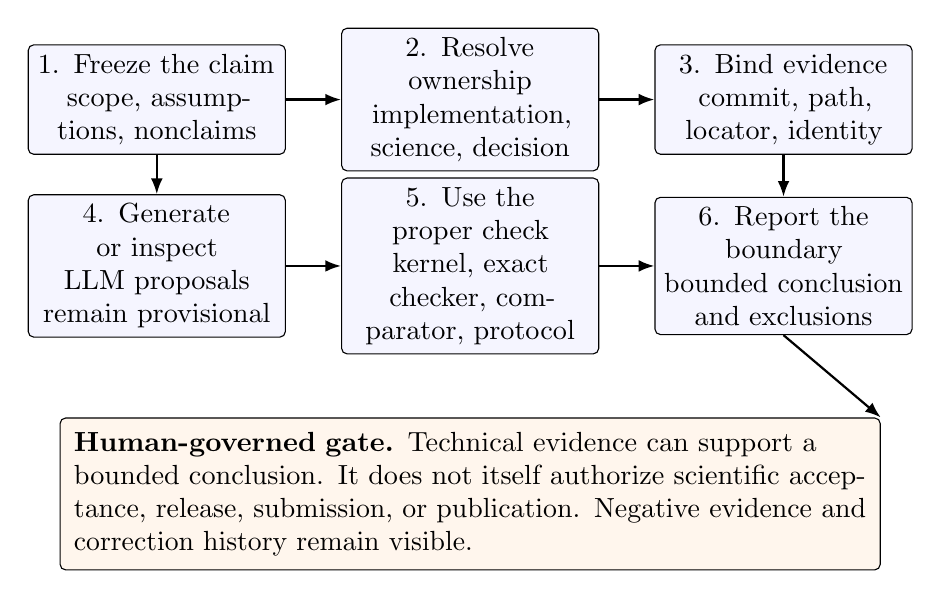
\begin{tikzpicture}[
  node distance=5mm and 7mm,
  box/.style={
    draw,
    rounded corners=2pt,
    align=center,
    text width=0.25\linewidth,
    minimum height=12mm,
    fill=blue!4
  },
  boundary/.style={
    draw,
    rounded corners=2pt,
    align=left,
    text width=0.83\linewidth,
    inner sep=5pt,
    fill=orange!7
  },
  arrow/.style={-{Latex[length=2mm]}, thick}
]
  \node[box] (claim) {1. Freeze the claim\\scope, assumptions, nonclaims};
  \node[box, right=of claim] (owner) {2. Resolve ownership\\implementation, science, decision};
  \node[box, right=of owner] (bind) {3. Bind evidence\\commit, path, locator, identity};

  \node[box, below=of claim] (assist) {4. Generate or inspect\\LLM proposals remain provisional};
  \node[box, right=of assist] (check) {5. Use the proper check\\kernel, exact checker, comparator, protocol};
  \node[box, right=of check] (report) {6. Report the boundary\\bounded conclusion and exclusions};

  \draw[arrow] (claim) -- (owner);
  \draw[arrow] (owner) -- (bind);
  \draw[arrow] (bind) -- (report);
  \draw[arrow] (assist) -- (check);
  \draw[arrow] (check) -- (report);
  \draw[arrow] (claim) -- (assist);

  \node[boundary, below=8mm of check] (gate) {
    \textbf{Human-governed gate.} Technical evidence can support a bounded
    conclusion. It does not itself authorize scientific acceptance, release,
    submission, or publication. Negative evidence and correction history remain
    visible.
  };
  \draw[arrow] (report.south) -- (gate.north east);
\end{tikzpicture}

  \caption{Audit-first claim admission. LLM-produced material remains
  provisional until the claim is bound to the appropriate evidence and its
  boundary is reported.}
  \label{fig:workflow}
\end{figure}

\paragraph{Freeze the claim.}
The intended conclusion, assumptions, domain, and exclusions are stated before
the artifact is treated as evidence. This prevents a successful computation
from expanding the claim after the fact.

\paragraph{Resolve ownership.}
The workflow distinguishes ownership of reusable implementation, retained
calculations, scientific meaning, and protected decisions. Repository transfer
does not automatically transfer campaign tolerances, execution authority,
material interpretation, or publication authority.

\paragraph{Bind immutable evidence.}
An admitted claim records an owner-repository semantic identity, public remote,
commit, repository-relative path, and line or declaration locator. Claim IDs,
evidence IDs, and artifact IDs remain distinct, so one claim can cite several
artifacts without flattening their roles.

\paragraph{Generate or inspect.}
An LLM may search bounded sources, propose code or proof terms, draft tests,
suggest classifications, and identify inconsistencies. Its output is a
proposal, not the acceptance event.

\paragraph{Apply the proper check.}
A formal proposition is checked by the pinned kernel; an exact certificate
requires exact data, a checker, and a proved bridge; a numerical claim requires
a declared comparator, tolerance, finite domain, and environment; scientific
validation requires scientific reference evidence and review. Human-governed
choices remain human decisions.

\paragraph{Report the boundary.}
The accepted statement is accompanied by explicit nonclaims. Failed attempts,
rejected prototypes, unresolved gaps, and deprecations remain visible. The
machine-readable ledger implements this structure for the case claims used by
the reviewed report \citep{projectkoios_ledger_2026}.

\section{Evidence and authority taxonomy}
\label{sec:taxonomy}

Table~\ref{tab:evidence} summarizes the evidence classes. The classes answer
what kind of conclusion an artifact can support; they do not encode release or
publication authority.

\begin{table}[htbp]
\centering
\small
\caption{Evidence classes and their principal boundaries.}
\label{tab:evidence}
\begin{tabular}{>{\raggedright\arraybackslash}p{0.24\linewidth}
                >{\raggedright\arraybackslash}p{0.34\linewidth}
                >{\raggedright\arraybackslash}p{0.34\linewidth}}
\toprule
Class & Bounded basis & Not implied \\
\midrule
Implementation conformance & Mapped behavior, contract, and tests at an
identified revision & Scientific adequacy, behavior outside the exercised
domain, or release approval \\
Lean theorem evidence & Exact proposition and proof term checked by the pinned
kernel, with assumptions and reported axioms & Source fidelity, runtime
correctness, numerical convergence, or physical applicability \\
Exact checked certificate & Exact data accepted by a checker connected by proof
to a target proposition & Correctness of unbound external files or
floating-point calculations \\
Numerical verification & Declared finite computation, comparator, tolerance,
and environment & Exact equality, continuum behavior, uncertainty
quantification, or material validation \\
Scientific validation & Reference observation or artifact, applicability
domain, uncertainty treatment, protocol, and scientific review & Universal
validity or publication acceptance \\
Experience observation & Immutable record of a bounded occurrence and its
limitations & Recurrence, general effectiveness, or promotion into another
class \\
Planned work & Explicit future protocol or requirement & Implementation,
execution, verification, or completion \\
\bottomrule
\end{tabular}
\end{table}

Authority is a separate dimension. Claim acceptance, scientific interpretation,
execution authorization, release, and publication are not evidence classes.
Figure~\ref{fig:separation} illustrates the separation. A technically adequate
artifact can coexist with a pending human decision, and a human decision cannot
create a mathematical or numerical result merely by accepting it.

\begin{figure}[htbp]
  \centering
  % Reviewable vector source; included by Ragasa2026_pk_a.tex.
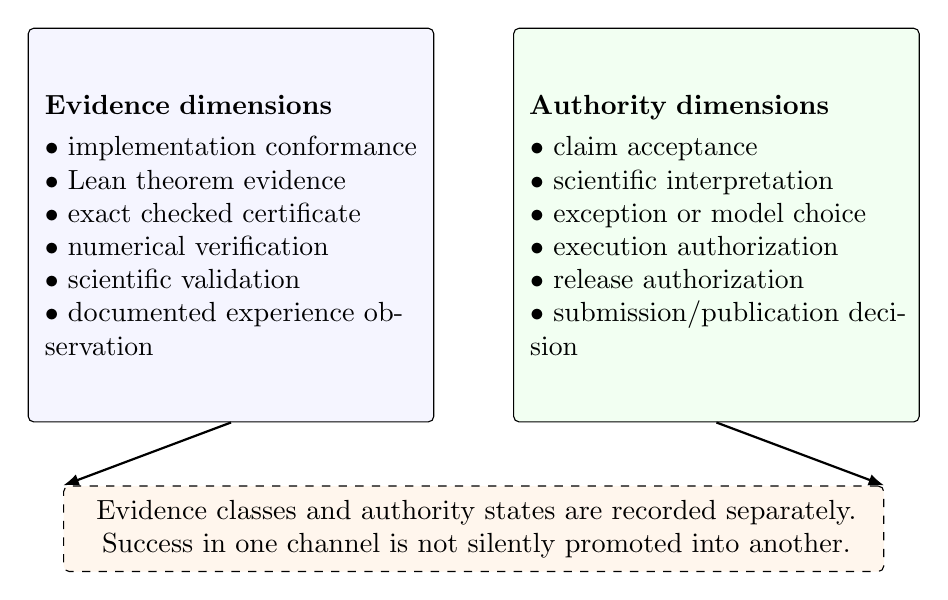
\begin{tikzpicture}[
  column/.style={draw, rounded corners=2pt, align=left, text width=0.39\linewidth,
    inner sep=6pt, minimum height=50mm},
  note/.style={draw, dashed, rounded corners=2pt, align=center,
    text width=0.83\linewidth, inner sep=5pt, fill=orange!7},
  arrow/.style={-{Latex[length=2mm]}, thick}
]
  \node[column, fill=blue!4] (evidence) {
    \textbf{Evidence dimensions}\par\smallskip
    $\bullet$ implementation conformance\par
    $\bullet$ Lean theorem evidence\par
    $\bullet$ exact checked certificate\par
    $\bullet$ numerical verification\par
    $\bullet$ scientific validation\par
    $\bullet$ documented experience observation
  };
  \node[column, fill=green!5, right=10mm of evidence] (authority) {
    \textbf{Authority dimensions}\par\smallskip
    $\bullet$ claim acceptance\par
    $\bullet$ scientific interpretation\par
    $\bullet$ exception or model choice\par
    $\bullet$ execution authorization\par
    $\bullet$ release authorization\par
    $\bullet$ submission/publication decision
  };
  \node[note, below=8mm of $(evidence.south)!0.5!(authority.south)$] (boundary) {
    Evidence classes and authority states are recorded separately. Success in
    one channel is not silently promoted into another.
  };
  \draw[arrow] (evidence.south) -- (boundary.north west);
  \draw[arrow] (authority.south) -- (boundary.north east);
\end{tikzpicture}

  \caption{Evidence and authority are recorded as separate dimensions. No arrow
  denotes automatic promotion from one item to another.}
  \label{fig:separation}
\end{figure}

\section{Role and limits of LLM assistance}
\label{sec:llm}

Within the workflow an LLM can assist with discovery, decomposition, drafting,
implementation, formal proof search, test construction, and editorial review.
The \texttt{ksdft2effmass} monograph source discloses assistance with drafting,
code, analysis, and editorial work while assigning scientific selection,
interpretation, reporting, and responsibility to the author
\citep{ksdft2effmass_2026}. The cited Formal proof dossier similarly labels a
bounded result AI-assisted and kernel-checked \citep{projectkoios_formal_2026}.

The checker, retained artifact, and accountable person---not the model's
rhetorical confidence---carry authority. In particular, an LLM cannot merely by
generating text:

\begin{itemize}
  \item declare its own theorem correct;
  \item convert approximate output into an exact certificate;
  \item choose an undisclosed tolerance, model, or applicability domain;
  \item promote a software test into scientific validation;
  \item authorize execution, release, submission, or publication; or
  \item erase a failed attempt and retain only the corrected endpoint.
\end{itemize}

This article does not expose private transcripts or hidden reasoning. Such
material is neither necessary nor sufficient for reproducing the admitted
claims. Reproducibility instead rests on public artifacts, immutable identities,
and explicit check boundaries. No controlled comparison supports a productivity
or quality-benefit claim, and no evidence establishes universal compliance by
an LLM with prompts, policy, or scientific norms.

\section{Case studies}
\label{sec:cases}

\subsection{Formal: Lean theorem evidence and an exact analytic certificate}

At public Formal checkpoint
\texttt{26603110e9d64cd51c9101eff68060307f258a18}, Lean is pinned to
version 4.35.0 and Mathlib to an immutable revision
\citep{projectkoios_formal_2026}. The encoded two-observation Paper A
construction has a proved declaration whose conjunction states zero canonical
spectral loss at the encoded witness, membership in the spectral pass set,
positive scale, and disjointness from an optimized-operator pass set. The owner
records report the axioms and explicit boundaries.

A separate but connected evidence channel contains exact rational data, a
Boolean rational-enclosure checker, checker-soundness theorems, and
source-specific bridge theorems. This supports one exact analytic
source-certificate chain for the encoded construction. It is important not to
collapse the two channels: a Lean theorem and an exact checked certificate are
related here, but they answer different audit questions.

\nonclaim{The checkpoint does not contain a runtime data/parser certificate
binding. The exact source certificate does not bind external floating-point
artifacts, prove source fidelity, validate a material, or establish a continuum
claim. This manuscript does not claim that Lean was rerun during its
preparation.}

\subsection{Optimization and numerics: provisional source definitions}

The public migration-branch checkpoint
\texttt{b722edab216ef416b8b4affa902b04a26e3da98b} documents bounded
finite-periodic transforms, evaluation, diagnostics, and optimization
capabilities while assigning scientific coordinates, units, thresholds, and
acceptance to consumers \citep{projectkoios_optimization_2026}. Its package
metadata records development version \texttt{0.1.0.dev0}. It is treated here as
provisional source, not a tag, release, or adopted downstream baseline.

Source inspection shows that one finite-series test defines one-, two-, and
three-dimensional comparisons against a direct Fourier sum evaluated inside
\texttt{mpmath.workdps(100)}. Each reference real and imaginary component is
converted to binary64 before comparison, and the source defines an explicit
floating-point acceptance bound. Other source tests define reconstruction,
Parseval, and Hermiticity checks with explicit bounds. A correction commit adds
an independently declared Hermiticity-defect case.

These are source-level test definitions for prospective numerical verification.
No retained command or CI artifact is admitted as an executed
numerical-verification result for this checkpoint. The definitions are not
exact certificates or scientific validation, and the library does not select
consumer scientific tolerances.

\subsection{PhysKit: consistency procedures and provenance boundaries}

At public PhysKit checkpoint
\texttt{11e58938ac8d0022f9e6df3aba7ca8757b4a9f88}, package metadata records
development version \texttt{0.1.3.dev0}; the checkpoint is not presented as a
release \citep{projectkoios_physkit_2026}. A Morse-potential test source checks
force directions and defines a consistency procedure for
$F_r=-\mathrm{d}V/\mathrm{d}r$. It compares the returned radial force with a
separately expressed centered finite-difference approximation formed from the
returned production potential energies, using step $10^{-5}$ angstrom,
relative tolerance $5\times10^{-10}$, and zero absolute tolerance.

The procedure is not producer-independent: force and energy are returned by the
same production evaluator. Moreover, source inspection is not a retained
executed result. A periodic-cosine provenance record classifies its mapped
checks as implementation and numerical verification while explicitly excluding
experimental validation of a material potential.

PhysKit also records a rejected oblique-periodic notebook prototype. Clean
execution stopped at a syntax error, saved displays could not be reproduced
from the source, and invalid behavior was not migrated. Exact bytes remained
recoverable after maintained replacement. This documents review, rejection,
correction, and byte-level preservation; it does not document an exercised
rollback or a general rollback mechanism.

Extraction records preserve donor identities while retaining campaign
tolerances, retained calculations, execution authority, semiconductor-specific
interpretation, scientific-validation conclusions, and human acceptance with
\texttt{ksdft2effmass}. Reusable represented mathematics can move without
silently moving those authorities.

\subsection{KSD: retained finite numerical experiments}

At public \texttt{ksdft2effmass} checkpoint
\texttt{5aaff25b784c7d1bc079a3030a73be387dc11a0f}, the retained
particle-in-a-box case is explicitly an illustrative numerical experiment, not
a public API, software harness, semiconductor calculation, or material-
validation result \citep{ksdft2effmass_2026}. A 38-entry SHA-256 manifest
supports maintained-file identity. The reviewed claim uses that manifest only
for identity and makes no same-checkpoint producer-script causality claim.

Retained independent verifiers compare finite results against declared
finite-difference oracles, projector identities, and residual identities under
binary64 arithmetic. Fixed low modes display the expected second-order trend
for the declared grids, while modes whose index scales with grid dimension do
not show uniform eigenvalue accuracy. This is bounded numerical verification of
the finite illustrative construction. It is not evidence about silicon, DFT,
Wannier localization, impurity physics, or a material model.

A deprecation record freezes historical Stage C interfaces and exact bytes,
names newer adapters, and transfers no scientific, numerical-policy, or
execution authority. A separate composite-band successor remains marked
\texttt{MIGRATION\_IN\_PROGRESS}; it has no admitted immutable experiment
version, maintained run, or new result.

\subsection{Pi coordination harness: candidate mechanics and a retained failure}

At public Bootstrap checkpoint
\texttt{7fa09bc3b631984d3b049b00d858935575d5687d}, the accepted incubation
boundary permits bounded source, sanitized fixtures, tests, and limitations
while excluding transcripts, generated handoffs, credentials, and runtime
state \citep{projectkoios_bootstrap_2026}. Candidate documents specify
deterministic preflight, explicit repository and task naming, fail-closed scoped
messaging checks, bounded failures, and the absence of a durable orchestration
database. Mocked or fake-boundary test coverage does not prove a live Pi or Herdr
service, model compliance, or an authorization service.

A retained incident records that a pane was closed instead of the client being
detached, terminating the Pi process. A read-only continuity diagnostic fails
closed but cannot recover a terminated process; reassignment remains an
authorized human action. The incident supports a bounded experience observation,
not autonomous rollback, recurrence, or end-to-end availability.

\section{Failures and corrections as evidence}
\label{sec:failures}

An audit-first account retains negative evidence because it constrains what can
be claimed and makes corrections inspectable. Across the cases, the relevant
records include:

\begin{itemize}
  \item an exact formal counterexample as a primary mathematical result rather
  than a failed success case;
  \item replacement of a correlated diagnostic assertion by an independently
  declared test input;
  \item rejection of a notebook whose saved displays were not reproducible from
  clean execution;
  \item deprecation that preserves historical interfaces and byte identities
  without rewriting provenance; and
  \item an operational pane-loss incident that motivated a bounded read-only
  diagnostic rather than an autonomous recovery claim.
\end{itemize}

These records do not establish a general rollback system, a correction success
rate, or a recovery-time distribution. Their narrower contribution is to keep
the path from defect to bounded correction visible. Availability of historical
bytes is not the same as an exercised rollback.

\section{Threats to validity}
\label{sec:threats}

\paragraph{Selection and survivorship.}
The cases were selected from one repository family and were not randomly
sampled. Repository-visible failures may omit private, informal, abandoned, or
undocumented work. No failure rate or general effectiveness estimate follows.

\paragraph{Independence.}
Many artifacts were authored, reviewed, or selected by the same project owner.
A separately expressed comparator can reduce some correlated errors, but common
libraries, assumptions, and authorship remain. Kernel checking is not
independent scientific peer review. The PhysKit Morse consistency procedure
uses values from the same production evaluator and is explicitly not called
producer-independent verification.

\paragraph{Evidence freshness and branch semantics.}
Commits are immutable, but statements about current project state can become
stale. Branch reachability does not establish release or adoption. The
Optimization case is explicitly provisional, and the KSD commit being reachable
from public main does not establish publication or release status.

\paragraph{Tool and model reproducibility.}
Model behavior can depend on provider, version, prompt, context, tools, and
sampling. The method does not promise byte-reproducible model reasoning. It
instead freezes accepted public artifacts. Tool availability and dependency
resolution can still affect a later rerun.

\paragraph{Scientific reach.}
The cases concern formal statements, source-level test definitions, finite
illustrative calculations, and selected engineering records. They do not
validate semiconductor materials, DFT approximations, experimental observables,
or multiscale predictive use.

\paragraph{Productivity.}
No predeclared baseline task set, blinded comparison, complete time/cost record,
or controlled study exists. Commit counts, passing tests, token counts, and
anecdotal speed cannot support a productivity conclusion.

\section{Reproducibility and evidence availability}
\label{sec:reproducibility}

The reviewed narrative and ledger are publicly addressable at exact Project
Koios commit \texttt{45da16e6428c3c431359da4f80f46de7ebf71081}
\citep{projectkoios_report_2026,projectkoios_ledger_2026}. The ledger separates
37 claim identities from 33 evidence records and 37 artifact identities. Each
artifact record includes an owner repository, public remote, commit,
repository-relative path, and exact line locators. The manuscript cites the
owner checkpoints rather than copying their source.

The canonical manuscript source is \texttt{Ragasa2026\_pk\_a.tex}. TikZ figures
are retained as reviewable vector source. The local build writes auxiliary files
under \texttt{.build/}; the rendered PDF retained beside the source is a Draft
artifact, not a release. Build-tool identity and the PDF digest are recorded in
the publication README.

Reproducing a bounded claim requires consulting the corresponding ledger record,
not merely rebuilding this PDF. The PDF is a readable projection of the method;
it is not the evidence database and does not promote planned or source-only
items into completed results.

\section{Rights, authorship, and ethics}
\label{sec:rights}

The author line is provisional. Affiliation, correspondence, contributor roles,
and final authorship require human confirmation. LLM assistance receives neither
authorship nor scientific authority merely because text or code was generated.
The human author remains responsible for claim selection, interpretation,
citations, rights, disclosure, and any future submission decision.

Rights review for a future deposit remains pending. The cited owner repositories
contain license and notice records, including repository-specific third-party
and adaptation notices. Those records do not establish redistribution
permission for every cited or depositable file. This source links to public
artifacts and does not vendor owner code, retained scientific data, or protected
publication expression.

No private filesystem paths, credentials, session transcripts, hidden runtime
state, private benchmark payloads, or unpublished scientific results are
included. The work reports software and research-method experience; it does not
report a human-subject experiment or use an LLM output as a human acceptance
decision. Venue-specific authorship, disclosure, ethics, and rights requirements
must be rechecked before any submission.

\section{Conclusion}

The \projectkoios{} experience supports a narrow methodological conclusion:
selected public artifacts demonstrate a practice of separating LLM assistance
from formal checking, exact certificate checking, source-level numerical test
definitions, retained numerical verification, scientific interpretation, and
human-governed decisions. The repositories also preserve selected failures,
corrections, and deprecated paths.

The evidence does not establish material validation, universal LLM compliance,
productivity benefit, peer review, release, or publication acceptance. The
value of the workflow lies in making these boundaries inspectable: each admitted
claim is narrower than the set of plausible statements an LLM could draft, and
each unresolved authority remains explicit.

\begingroup
\raggedright
\setlength{\bibsep}{0.5\baselineskip}
\bibliographystyle{plainnat}
\bibliography{references}
\endgroup

\end{document}
